\documentclass[
	12pt,
	BCOR=5mm,
	DIV=12,
	headinclude=on,
	footinclude=off,
	parskip=half,
	bibliography=totoc,
	listof=entryprefix,
	toc=listof,
	pointlessnumbers,
	plainfootsepline]{scrreprt}

\input{config}

\begin{document}

%% BITTE GEBEN SIE HIER DEN TITEL UND DIE AUTORIN / DEN AUTOR DER ARBEIT AN!
%% DIESE INFORMATIONEN _MÜSSEN_ GESETZT SEIN, UM TITELBLATT, ABSTRACT UND
%% EIGENSTÄNDIGKEITSERKLÄRUNG AUTOMATISCH ANZUPASSEN!
\TitelDerArbeit{Projekt ExoPlan: Entwicklung eines Vorlesungsverwaltungstools}
\AutorDerArbeit{Kurs WWI 17 SE B}

\begin{titlepage}
\begin{minipage}{\textwidth}
		\vspace{-1cm}
        \begin{center}
            \includegraphics[scale=1.5]{img/logo.jpg}
        \end{center}
\end{minipage}
\vspace{4em}
\sffamily

\begin{center}
	\textsf{\Large{}Duale Hochschule Baden-W\"urttemberg\\[1.5mm] Mannheim}\\[4.5em]
	\textsf{\Large{}Dokumentation}\\[3mm]
	\textsf{\textbf{\Large{}\DerTitelDerArbeit}} \\[2.5cm]
	\textsf{\Large{}Studiengang Wirtschaftsinformatik}\\[3mm] \textsf{Studienrichtung Software Engineering}
	\vspace{2em}
\vfill

\begin{minipage}{\textwidth}

\begin{tabbing}
    Wissenschaftlicher Betreuer: \hspace{0.85cm}\=\kill
	Verfassende: \> \DerAutorDerArbeit \\[2mm]
	Studiengangsleiter: \> Prof. Dr. Sebastian Ritterbusch  \\[2mm]
	Dozent: \> Tarek Becker \\
	\> tarek@becker.ly \\[2mm]
	Bearbeitungszeitraum: \> 20.11.2019 -- 02.08.2020
\end{tabbing}
\end{minipage}

\end{center}
\end{titlepage}

\pagenumbering{roman} % Römische Seitennummerierung
\normalfont

%--------------------------------
% Verzeichnisse - nicht benötige Verzeichnisse bitte auskommentieren / löschen.
%--------------------------------

%	Inhaltsverzeichnis
    \tableofcontents

% %	Abbildungsverzeichnis
% \listoffigures
% \listoftables
% \lstlistoflistings
% \listofalgorithms

% 	Abkürzungsverzeichnis (siehe Datei acronyms.tex!)
\clearpage
\chapter*{Abkürzungsverzeichnis}
\addcontentsline{toc}{chapter}{Abkürzungsverzeichnis}


\begin{acronym}[A23456789]
	\acro{A23456789}{This is just for indentation}
	
	\acro{API}{Application Programming Interface}
	\acrodefplural{API}[APIs]{Application Programming Interfaces}
	\acro{CSS}{Cascading Style Sheets}
	\acro{DHBW}{Duale Hochschule Baden-Württemberg}
	\acro{DOM}{Document Object Model}
	\acro{HTML}{Hypertext Markup Language}
	\acro{HTTP}{Hypertext Transfer Protocol}
	\acro{HTTPS}{Hypertext Transfer Protocol Secure}
	\acro{ORM}{Objektrationales Mapping}
	\acro{RDBMS}{Relational Database Management System}
	\acro{REST}{Representational State Transfer}
	\acro{SPA}{Single-Page-Application}
\end{acronym}

\ohead{Acronyms} % Neue Header-Definition

%--------------------------------
% Start des Textteils der Arbeit
%--------------------------------
\clearpage
\ihead{\chaptername~\thechapter} % Neue Header-Definition (inner header)
\ohead{\headmark} % Neue Header-Definition (outer header)
\pagenumbering{arabic}  % Arabische Seitenzahlen

\chapter{Einleitung}
Die vorliegende Dokumentation soll einen Überblick über das Projekt, dessen Verlauf sowie die finalen Ergebnisse geben.
In den verschiedenen Kapiteln wird zunächst das Projektziel vorstellt und anschließend der Entwicklungsprozess der erstellten Software erläutert.

Zunächst ist im Kapitel \nameref{ch:Projektmanagement} die Organisation des Projekts und des Projektteams beschrieben.
Anschließend folgt das Einholen der Anforderung und ihre Priorisierung in der \nameref{ch:Anforderungsanalyse}.
Im \nameref{ch:Entwurf} wird sowohl der \nameref{ch:DesignEntwurf} als auch der \hyperref[ch:Technischer Entwurf]{Technische Entwurf} beschrieben.

Die \nameref{ch:Umsetzung} geschildert Infrastruktur des Verwaltungstools, die Umsetzung des Back-Ends sowie Front-Ends und anschließende Tests.
Darüber hinaus wird in einem \nameref{ch:UserGuide} das Aufsetzen der Software und deren Benutzung erläutert.

Schließlich werden in der \nameref{ch:Evaluation} die Anforderungen und deren Umsetzung gegenübergestellt, sowie die Lernerfolge und nächsten Schritte beschrieben.
Abschließend wird ein Fazit zu dem Projektergebnis sowie dem Projektablauf gezogen.
Darüber hinaus wird ein Ausblick bezüglich zukünftigen Entwicklungen gegeben.
Im Anhang sind außerdem vertiefende Inhalte beigefügt.
\chapter{Projektmanagement}
\label{ch:Projektmanagement}
\section{Projektdefinition}
- Projektziel 
- Beschreibung des Projekts

\section{Projektbeteiligte}
Zu den Beteiligten des Projekts gehört zunächst das Projektteam, welches aus dem Kurs WWI17SEB der DHBW Mannheim besteht.
Dieses ist für die Umsetzung der Anwendung zuständig, weshalb das Team zu Beginn des Projekts in verschiedene Aufgabenbereiche und Zuständigkeiten aufgeteilt wurde.
Die genaue Aufteilung kann dem Organigramm in Abbildung \vref{fig:Organigramm} entnommen werden.
Eine detailliertere Beschreibung der jeweiligen Aufgaben folgt in Kapitel \vref{ch:Teamorganisation}. 

\begin{figure}[h]
	\centering 
	\includegraphics[width=12cm]{img/Organigramm.pdf}
	\captionsetup{format=hang}
	\caption[Organigramm des Projektteams]{\label{fig:Organigramm}Organigramm des Projektteams}
\end{figure}

Weitere Beteiligte des Projekts sind die Stakeholder.
Dazu zählen Prof. Dr. Matt, Prof. Dr. Ritterbusch und Prof. Dr. Reichwald, welche die Kunden der Anwendung sind.
Die Betreuung und Bewertung des Projekts erfolgt durch Herrn Becker.



 


\section{Zeitplanung}
Für die Planung und Kontrolle des Projektfortschritts wurde pro Semester ein Zeitplan erstellt.
Die Gantt-Diagramme des 5. und 6. Semesters geben einen groben Überblick über diese.
Für das 5. Semester (siehe Abbildung \vref{fig:Gantt5}) wurden verschiedene Zeiträume aufgestellt jedoch ohne inhaltliche Ziele.
Dem Zeitplan des 6. Semesters (siehe Abbildung \vref{fig:Gantt6}) wurden für die jeweiligen Zeitabschnitte inhaltliche Ziele hinzugefügt, wodurch der Fortschritt des Projekts besser kontrolliert werden konnte.

\begin{figure}[H]
	\centering 
	\includegraphics[width=\textwidth]{img/GanttSemester5.png}
	\captionsetup{format=hang}
	\caption[Grobe Übersicht Gantt-Diagramm Semester 5]{\label{fig:Gantt5}Grobe Übersicht Gantt-Diagramm Semester 5}
\end{figure}

\begin{figure}[H]
	\centering 
	\includegraphics[width=\textwidth]{img/GanttSemester6.png}
	\captionsetup{format=hang}
	\caption[Grobe Übersicht Gantt-Diagramm Semester 6]{\label{fig:Gantt6}Grobe Übersicht Gantt-Diagramm Semester 6}
\end{figure}

\section{Teamorganisation}
Zunächst wurde als Projektleiter Kay Wessel festgelegt, der die gesamte Verantwortung für das Projekt trägt und deshalb die oberste Entscheidungsgewalt inne hat. 
Zu seinen Aufgaben gehört die Gesamtplanung des Projekts und das Managen von organisatorischen Angelegenheiten, wie Aufsetzen und Durchführung von Meetings sowie das Klären von inhaltlichen Fragen.
\\Für das Projekt konnten die drei Aufgabenbereichen Produktmanagement, Front-End und Back-End identifiziert werden.
Anhand dieser Aufgabenbereiche wurde der Kurs in drei dedizierte Teams unterteilt, welche jeweils der Führung eines Teamleiters unterliegen.
Für das Produktmanagement ist Kay Wessel zuständig, Sandra Keller für das Front-End und Martin Sandig für das Back-End.
Die Aufgabe der Teamleiter ist die Verteilung und Kontrolle von Aufgaben unter den jeweiligen Mitgliedern eines Teams.
Das Planen und Erfassen der Aufwände fällt ebenfalls in ihren Tätigkeitsbereich.

Die Organisation und Realisierung des Projektes erfolgte mittels der Nutzung unterschiedlicher digitaler Medien.
Als Unterstützung agiler Softwareentwicklung wurden GitHub sowie Trello verwendet. 
Der netzbasierter Dienst \textit{GitHub}\footnote{\url{https://github.com/}} ermöglicht gemeinsames Arbeiten und die Versionsverwaltung bei Software-Entwicklungsprojekten. 
Für die Entwicklung des Front-End und Back-End sowie für die Erstellung der Dokumentation werden eigene Verzeichnisse (Repositories) verwendet. 
\\Der Aufgaben-Verwaltungs-Onlinedienst \textit{Trello}\footnote{\url{https://trello.com/}} ermöglicht das Verwalten von Aufgaben in sogenannten Boards. 
Die Aufgaben können beliebig bearbeitet und mit Checklisten, Anhängen, Terminen und vielem mehr versehen werden.
Außerdem lassen sich die Bearbeiter zu einer Aufgabe hinzufügen, sodass diese über alle Änderungen und Fortschritte informiert werden.
Für jedes Team wurde in Trello ein eigenständiges Board erstellt, sodass die Aufgaben im Verbund eines Teams entsprechend zugeordnet und anschließend bearbeitet werden können. 
Zur Klärung allgemeiner Fragen wurde ein gemeinsames Board \enquote{Organisation} eingerichtet.
Da für das Projekt eine Protokollierung der Stunden erforderlich ist, wurde ein geteiltes \textit{Google-Sheet}\footnote{\url{https://www.google.com/sheets/about/}} erstellt, welches das aktuelle Stundenkontingent der Teammitglieder beinhaltet. 
Dieses und die Aufgabenverwaltung mit Trello gewährleisten die Transparenz über die aktuellen Aufwände und Aufgaben. 
\\Die Kommunikation und Koordination erfolgte über den Instant-Messaging-Dienst \textit{WhatsApp}\footnote{\url{https://www.whatsapp.com/}} sowie das Konferenzsystem \textit{Discord}\footnote{\url{https://discord.com/}}.
In Letzterem sind verschiedene Sprachkanäle eingerichtet, in denen telefonische Absprachen durchgeführt werden können.
Dabei besteht die Möglichkeit den Bildschirm und damit Inhalte zu teilen, welches unter anderem für das gemeinsame Bearbeiten von Aufgaben genutzt wurde. 


\section{Interne Aufgabenverteilung}
- regelmäßigen Meetings
- Springer für FE und BE 

\input{tex/Projektmanagement/Projektabschluss.tex}

\chapter{Anforderungsanalyse}

%\chapter{Anforderungsanalyse}
\label{ch:Anforderungsanalyse}

In diesem Kapitel wird die Anforderungsanalyse erstellt.
Zunächst wird die zu lösende Problemstellung sowie die Zielsetzung des Projekts beschrieben.
Anschließend werden die Anforderungen des Auftraggebers identifiziert.
Alle Anforderungen werden danach anhand ihrer Relevanz und dem gegebenen zeitlichen Budget priorisiert.


\section{Problemstellung und Zielsetzung}\label{sec:probl}

Die Vorlesungspläne für die Kurse des Studiengangs Wirtschaftsinformatik an der \ac{DHBW} müssen aktuell vollständig manuell durch die jeweiligen Tutoren erstellt werden.
Eine Excel-Vorlage dient dabei als Unterstützung, indem darin Informationen über den Kurs und die Module gesammelt werden.
Für die zu haltenden Vorlesungen müssen passende Dozenten gesucht und angefragt werden, wobei keine zentrale Liste der Dozenten existiert, was den Prozess wiederum erschwert.
Wurden zu allen Vorlesungen passende Dozenten sowie Zeitfenster gefunden, werden diese in einem Google Calendar integriert.

Mit Hilfe eines Tools soll künftig das eben beschriebene Vorgehen zur Erstellung der Vorlesungspläne mit seinen manuellen Teilprozessen für die Studiengangsleiter erleichtert werden.
Ziel dabei ist es, eine zentrale Dozentenverwaltung zu realisieren sowie den Studiengangsleitern ein einheitliches System zur Planung und Koordination ihrer Kurse zur Verfügung zu stellen.

\section{Ist-Analyse}
%TODO


\section{Anforderungen}

Bevor der Lösungsansatz für die Problemstellung aus Kapitel \vref{sec:probl} konzipiert wird, müssen die Wünsche und Vorstellungen des Auftraggebers ermittelt werden.
Bei dem Auftraggeber handelt es sich um einen Studiengangsleiter des Studiengangs Wirtschaftsinformatik an der \ac{DHBW}.
Durch verschiedene Interviews wurden die Anforderungen des Auftraggebers festgestellt.
Die Anforderungen sind in Tabelle \ref{tab:Anforderungen} aufgelistet.

\begin{longtable}[h]{|p{2,5cm}|p{4cm}|p{6,5cm}|}		
	\multicolumn{3}{|r|}{\textit{Fortsetzung nächste Seite}} \\ \hline
	\endfoot
	\endlastfoot
	\hline &&\\[-0.5em]
	\textbf{Anforderung} & \head{Kurztitel} & \head{Beschreibung} \\ \hline
	\endfirsthead
	\hline &&\\[-0.5em]
	\textbf{Anforderung} & \head{Kurztitel} & \head{Beschreibung} \\ \hline
	\endhead
	\parbox[t]{3cm}{A1} & Dozentenpool & Alle Dozenten sollen in einem zentralen Dozentenpool verwaltet werden können.\label{anf:Dozenten}\\ \hline
	\parbox[t]{3cm}{A2} & Stundenplan & Die Software soll Stundenpläne verwalten und erzeugen anhand diverser Parameter, die eingetragen werden wie z.\,B. welche Vorlesungen in welchem Semester für einen Kurs und Dozenten stattfinden.\\ \hline
	\parbox[t]{3cm}{A3} & Google Calendar & Google Calendar soll vollständig in die Software integriert werden.\label{anf:GC}\\ \hline
	\parbox[t]{3cm}{A4} & Profilzuordnung & Die Profile der User, mit denen sie sich am System anmelden, sollen über deren  Mail-Adresse zugeordnet werden.\label{anf:Profilzuordnung}\\ \hline
	\parbox[t]{3cm}{A5} & Modulkataloge & Die Modulkataloge mit den Vorlesungen, Stundenanzahlen und Prüfungsmöglichkeiten (Klausur, Referat oder andere Ausarbeitungen) sollen verwaltet und über Templates hinzugefügt werden können.\label{anf:Modulkatalog} \\ \hline
	\parbox[t]{3cm}{A6} & Kurskoordination & Ein Studiengangsleiter soll eine variable Anzahl an Kursen im System koordinieren können.\\ \hline
	\parbox[t]{3cm}{A7} & Eindeutigkeit der Module & Module müssen eindeutig identifizierbar sein, da z.\,B. das Statistikmodul für Wirtschaftsinformatiker nicht gleich dem Statistikmodul für angewandte Informatiker ist.\\ \hline
	\parbox[t]{3cm}{A8} & Suchen und Filtern im Dozentenpool & In dem Dozentenpool sollen Dozenten per Suche gefunden sowie nach sinnvollen Kriterien gefiltert werden können.\\ \hline
	\parbox[t]{3cm}{A9} & Hinzufügen und Löschen im Dozentenpool & In dem Dozentenpool sollen neue Dozenten hinzugefügt und bestehende Dozenten gelöscht werden können.\\ \hline
	\parbox[t]{3cm}{A10} & Dozenteninformationen im Dozentenpool & Zu jedem Dozenten im Dozentenpool sollen Informationen wie Name, Mail, Handynummer verfügbar sein. Zudem sollen Felder für eine Bewertung, eine Information, ob der Dozent hauptamtlich tätig ist und der/die jeweilige(n) Schwerpunkt(e) sowie ein Freitextfeld für Kommentare vorhanden sein.\\ \hline
	\parbox[t]{3cm}{A11} & Automatisierte Dozentenanfrage & Nach Auswahl eines Dozenten soll diesem automatische eine Anfrage via Mail geschickt werden, wobei ein personalisierbares Template als Basis dient.\\ \hline
	\parbox[t]{3cm}{A12} & Zuordnung der Dozenten & Die Dozenten sollen jeweils einem Studiengangsleiter zugeordnet werden.\\ \hline
	\parbox[t]{3cm}{A13} & Warnung bei maximaler Studenanzahl & Das Tool soll benachrichtigen, wenn ein Dozent seine maximale Stundenanzahl überschreiten würde bei der aktuellen Planung.\\ \hline
	\parbox[t]{3cm}{A14} & Paralleler Zugriff & Parallele Zugriffe auf einen Kurs durch jeweils berechtigte Personen sollen möglich sein.\\ \hline
	\parbox[t]{3cm}{A15} & Tooladministration & Die Administration des Tools soll über die Studiengangsleiter erfolgen.\\ \hline
	\parbox[t]{3cm}{A16} & Kursübersicht & Es soll pro Kurs eine Übersicht mit Anzahl und Art der jeweiligen Prüfungsleistungen des Kurses existieren.\\ \hline
	\parbox[t]{3cm}{A17} & Farbiger Planungsstand & Der aktuelle Stand der Semesterplanung eines Kurses soll mithilfe von Farben verdeutlicht werden, z.\,B. grün – Termin der Vorlesung ist fix; gelb – Dozent hat zugesagt, aber noch kein fixer Termin; etc.\\ \hline
	\parbox[t]{3cm}{A18} & Planungsexport & Existierende Planungen sollen exportiert werden können, z.\,B. für nachfolgende Kurse.\\ \hline
	\parbox[t]{3cm}{A19} & Informationen der Veranstaltungen & Die detaillierten Informationen über die Veranstaltungen eines geplantes Kurses sollen mithilfe von angehängten Dokumenten einsehbar sein.\\ \hline
	\parbox[t]{3cm}{A20} & Veranstaltungstitel & Der Titel einer Veranstaltung soll in folgender Form dargestellt werden: \enquote{Name der Veranstaltung - Name des Dozenten}.\\ \hline
	\parbox[t]{3cm}{A21} & Automatisierte Benachrichtigungen & Kurse und Dozenten werden mit einer automatisch generierten E-Mail über Semesterbeginn, die finalisierte Planung  oder die Festlegung von Prüfungsterminen und -arten benachrichtigt.\\ \hline
	\parbox[t]{3cm}{A22} & Klausurenmaximum & Das Tool soll berücksichtigen, dass Studiengänge ab 2018  nur sechs schriftliche Klausuren pro Semester erlauben, indem eine entsprechende Warnung ausgegeben wird bei einer Überschreitung.\\ \hline
	\parbox[t]{3cm}{A23} & Korrekte Moduldurchführung  & Die Anwendung soll berücksichtigen, dass Lehrveranstaltungen eines Moduls innerhalb eines Studienjahres erfolgen müssen. Innerhalb eines Studienjahres sollen die Lehrveranstaltungen beliebig verschoben werden können.\\ \hline
	\parbox[t]{3cm}{A24} & Eintragung von Wahlmodulen & Wahlmodule sollen in den Modulkatalog eingetragen werden können.\\ \hline
	\parbox[t]{3cm}{A25} & Dozentenvorschläge & Bei neu hinzugefügten Modulen sollen Vorschläge für den Dozenten generiert werden.\\ \hline
	\parbox[t]{3cm}{A26} & Weiterführbarkeit & Die Software soll später von nachkommenden Jahrgängen weitergeführt und modifiziert werden können.\\ \hline
	\parbox[t]{3cm}{A27} & Usability & Die Bedienbarkeit der Software soll so intuitiv und einfach wie möglich gestaltet werden.\\ \hline
	
	\captionsetup{format=hang}
	\caption[Anforderungen des Auftraggebers]{\label{tab:Anforderungen}Anforderungen des Auftraggebers\\Quelle: Interview mit Professor Matt}
\end{longtable}


\section{Priorisierung}
Die Anforderungen werden, um sie zu priorisieren, in zwei Kategorien eingeteilt.
Als \textit{Muss} wird eine Anforderung kategorisiert, wenn sie die höchste Priorität hat.
Eine Nicht-Erfüllung einer Anforderung, die mit einem \textit{Muss}-Kriterium versehen wurde, kann die Ablehnung des gesamten Projektes oder Produktes bedeuten.
Die \textit{Kann}-Anforderungen sind Abstufungen der \textit{Muss}-Anforderungen und \enquote{können} erfüllt werden, soweit die Ressourcen dies ermöglichen.
Die Anforderungen mit ihren jeweiligen Priorisierungen sind in Tabelle \vref{tab:prios} dargestellt. 

\begin{table}[h]
	\centering
	\begin{tabular}{|l|p{8cm}|l|}
		\hline &&\\[-0.5em]
		\textbf{Anforderung} & \head{Kurztitel} & \textbf{Priorität} \\ \hline
		A1 & Dozentenpool & \textit{Muss} \\ \hline
		A2 & Stundenplan & \textit{Muss} \\ \hline
		A3 & Google Calendar & \textit{Muss} \\ \hline
		A4 & Profilzuordnung & \textit{Muss} \\ \hline
		A5 & Modulkataloge & \textit{Muss} \\ \hline
		A6 & Kurskoordination & \textit{Muss} \\ \hline
		A7 & Eindeutigkeit der Module & \textit{Muss} \\ \hline
		A8 & Suchen und Filtern im Dozentenpool & \textit{Muss} \\ \hline
		A9 & Hinzufügen und Löschen im Dozentenpool & \textit{Muss} \\ \hline
		A10 & Dozenteninformationen im Dozentenpool & \textit{Muss} \\ \hline
		A11 & Automatisierte Dozentenanfrage & \textit{Kann} \\ \hline
		A12 & Zuordnung der Dozenten & \textit{Kann} \\ \hline
		A13 & Warnung bei maximaler Stundenanzahl & \textit{Kann} \\ \hline
		A14 & Paralleler Zugriff & \textit{Kann} \\ \hline
		A15 & Tooladministration & \textit{Kann} \\ \hline
		A16 & Kursübersicht & \textit{Kann} \\ \hline
		A17 & Farbiger Planungsstand & \textit{Kann} \\ \hline
		A18 & Planungsexport & \textit{Kann} \\ \hline
		A19 & Informationen der Veranstaltungen & \textit{Kann} \\ \hline
		A20 & Veranstaltungstitel & \textit{Kann} \\ \hline
		A21 & Automatisierte Benachrichtigungen & \textit{Kann} \\ \hline
		A22 & Klausurenmaximum & \textit{Kann} \\ \hline
		A23 & Korrekte Moduldurchführung & \textit{Kann} \\ \hline
		A24 & Eintragung von Wahlmodulen & \textit{Muss} \\ \hline
		A25 & Dozentenvorschläge & \textit{Kann} \\ \hline
		A26 & Weiterführbarkeit & \textit{Kann} \\ \hline
		A27 & Usability & \textit{Muss} \\ \hline
	\end{tabular}
	\captionsetup{format=hang}
	\caption{\label{tab:prios}Priorisierung der Anforderungen \\}
\end{table}








\chapter{Entwurf}\label{ch:Entwurf}

\section{Design Entwurf}
%\begin{itemize}
%\item verwendetes Tool für die Mockups: figma.com; Gründe:
%	\subitem kostenlos für Studenten
%	\subitem man kann kooperativ in Echtzeit daran arbeiten
%	\subitem einfach zu bedienen
%	\subitem enthält alle wichtigen Design-Werkzeuge
%	\subitem man kann einen interkativen Prototypen erstellen
%\item Mitwirkende: 
%	\subitem Design-Team: Andrea, Verena
%	\subitem Qualitätssicherung: Falk
%\item Vorgehensweise
%	\subitem 1. Entwurf unterschiedlicher erster Design-Ideen
%	\subitem 2. Einholen der Anforderungen
%	\subitem 3. Auswahl einer ersten Design-Idee und deren Weiterentwicklung
%	\subitem 4. Erstellung eines interaktiven Prototypen aus den ersten Mockups
%\item Während des Design-Prozesses wurde immer wieder mit Falk Rücksprache gehalten.
%\end{itemize}

Für das Design sollte ein Prototyp erstellt werden, der den späteren Aufbau der Applikation verdeutlicht.
Als technisches Hilfsmittel wurde das cloud-basierte Tool \textit{Figma}\footnote{\url{https://www.figma.com/}} verwendet.
Dieses bietet die Möglichkeit mit mehreren Personen in Echtzeit an einem Prototypen zu arbeiten.
Dabei ist es in seiner Bedienung leicht verständlich und bietet alle wichtigen Design-Werkzeuge. 
Außerdem können die Elemente der Benutzeroberfläche miteinander verbunden und mit Interaktionen sowie Animationen versehen werden, sodass ein interaktiver Prototyp entsteht.
Nach dem Starten eines Prototyps kann das Design der Oberfläche sowie die Navigationen geprüft werden.
Über einen generierten Link lässt sich der Prototyp mit Projektbeteiligten teilen. 

Für das Erstellen des Designs wurde eine iterative Vorgehensweise gewählt.  
Gestartet ist der Prozess mit dem Einholen von Anforderungen.
Basierend darauf konnte die allgemeine Struktur der Benutzeroberfläche erstellt werden.
Anschließend verlief der Prozess in vielen Schleifen, in denen bekannte Anforderungen zunächst statisch umgesetzt und bei Rücksprachen mit den Stakeholdern deren Meinung eingeholt wurde.
Dabei wurden ebenfalls weitere Anforderungen besprochen, sodass das Design nachfolgend erweitert werden konnte.
Während den Schleifen wurden der Prototyp jeweils interaktiv erstellt und es wurden weitere Details hinzugefügt.
Auf diese Weise sind während dem Projekt verschiedene Versionen des Prototyps entstanden, die jeweils mit den Stakeholdern besprochen wurden.
Neben diesen Absprachen erfolgten Zusätzliche mit dem Backend-Team.
Thema dieser Besprechungen waren die geforderten Funktionalitäten, die vom Backend bereitgestellt werden müssen und die Umsetzbarkeit dieser.
Damit aber auch das gesamte Projektteam über den Entwurf und die Fortschritte informiert blieb, wurden das jeweils aktuelle Design in verschiedenen wöchentlichen Meetings des gesamten Teams präsentiert.
Damit jedes Team-Mitglied jederzeit auf den Prototyp zugreifen kann, wurde der Link in Trello eingetragen. 

%- Anforderungen eingeholt 
%- anfangs Struktur einer Seite erstellt 
%- erste Anforderungen zunächst statisch eingebaut 
%- Rücksprache mit Stakeholdern (Fragen oder Präsentation der Mockups)
%- Anschließend erfolgte das interaktive Erstellen der Mockups 
%- während Projekt weitere Anforderungen eingeholt, sodass Details zu den Mockups hinzugefügt werden konnten  
%- dadurch sind verschiedene Versionen von Mockups entstanden, die jeweils mit den Stakeholdern besprochen wurden 
%
%- neben den Rücksprachen mit Stakeholdern erfolgten ebenfalls Rücksprachen mit dem Backend bezüglich der geforderten Funktionalitäten und der Umsetzbarkeit dieser
%
%- Vorstellen in wöchentlichen Meetings oder Link teilen in Trello 

Die designte Benutzeroberfläche besteht, wie in Abbildung \ref{fig:Seitenaufbau} dargestellt, jeweils aus drei Elementen.
Sie beinhaltet eine Kopfzeile, eine Navigationsleiste und die gewählten Inhalte.
Die Kopfzeile stellt am linken Rand das Logo der \acs{DHBW} und am rechten Rand den Benutzernamen dar.
Durch das Anklicken des Benutzernamens können allgemeine Kontoeinstellungen getätigt oder das Abmelden von der Applikation ausgelöst werden.
Auf jeder Seite der Benutzeroberfläche befindet sich außerdem am linken Rand eine vertikale Navigationsleiste.
Diese beinhaltet die drei Hauptseiten und ermöglicht das Navigieren zwischen diesen.
Es können die Vorlesungen und Vorlesungspläne je Kurs angeschaut werden, eine Übersicht der Dozenten und verschiedene Modulkataloge. 

\begin{figure}[h]
	\centering 
	\includegraphics[width=\textwidth]{img/Seitenaufbau1.pdf}
	\captionsetup{format=hang}
	\caption[Aufbau der Benutzeroberfläche]{\label{fig:Seitenaufbau}Aufbau der Benutzeroberfläche}
\end{figure}

\textbf{Link finale Version Mockups}
\section{Technischer Entwurf}
\label{ch:Technischer Entwurf}
\subsection{Grundlegende Architektur}
\label{ch:grundlegendeArchitektur}
In Abbildung \vref{fig:Aufbau} ist der grundlengede Aufbau der Webanwendung skizziert.
Dieser besteht aus mehreren Komponenten, die gemäß eines Microservice-Ansatzes unabhängig voneinander bestehen. 
Dies bietet außerdem die Vorteile, dass durch die verringerte Kopplung eine bessere Wartbarkeit der einzelnen Bestandteile gegeben ist sowie diese einfach ersetzt werden können. 
Mithilfe eines Docker-Netzwerks kann dieser Ansatz umgesetzt werden und bietet zusätzlich ein einfaches Deployment der Anwendung. 

\begin{figure}[H]
	\centering 
	\includegraphics[width=13cm]{img/TechnischerEntwurf.pdf}
	\caption[Grundlegende Architektur]{\label{fig:Aufbau}Grundlegende Architektur}
\end{figure}

Die Abbildung stellt eine Übersicht über den Aufbau dar und bietet eine logische Trennung der Komponenten. 
Allgemein lassen sich folgende Hauptkomponenten unterscheiden:
\begin{itemize}
    \item Front-End zur Bereitstellung der Benutzeroberfläche an den Webbrowser des Clients 
    \item Back-End zur Datenhaltung und Geschäftslogik
    \item Proxy als Kommunikationsschnittstelle
    \item Webbrowser mit einer Anbindung an die Google Calendar-Schnittstelle.
\end{itemize} 

Das Front- und Back-End sollen als eigenständige Microservices mit eigenem Server umgesetzt werden, sodass die Entwicklung der Komponenten losgelöst ablaufen kann und durch andere Technologien ersetzt werden könnte.
Das Front-End dient zur Bereitstellung der grafischen Benutzeroberfläche und wird an den Webbrowser des Clients ausgeliefert. 
Das Back-End hingegen besteht aus einem Server mit der Geschäftslogik sowie einer Datenbank zur Datenhaltung der Anwendung. 
Diese Dienste sollen über eine \ac{API} erreichbar sein. 
Der Proxy stellt die zentrale Schnittstelle der Webanwendung dar und liefert das Front-End aus. 
Von dem Webbrowser wird außerdem auf die externe Schnittstelle des Google Calendars zugegriffen, um eine Verbindung zu einem Google Calendar gemäß der Anforderung A2 und A3 aus der Tabelle \ref{anf:GC} herzustellen.


\subsection{Datenmodell}
Für das serverseitige Speichern von Daten sind relationale Datenbanken weit verbreitet.
Deshalb wird auch im Rahmen dieses Projekts eine solche Form der Datenhaltung genutzt.
Im Folgenden wird nun das Datenmodell näher erläutert, welches im Anhang \vref{fig:ermodell} dargestellt ist.  

Über \texttt{directorOfStudies} werden die Nutzer der Anwendung, die Studiengangsleiter, dargestellt.
Sie sind nicht automatisch als Dozenten hinterlegt, können jedoch als solche hinzugefügt werden.
Ein Studiengangsleiter kann zusätzlich ein Administrator der Anwendung sein, wodurch er weitere Berechtigungen erhält, wie das Zurücksetzen von Passwörtern.

Die Entität \texttt{course} repräsentiert einen Kurs der \ac{DHBW}, welcher genau einem Studiengang (\texttt{fieldOfStudy}) und einer Studienrichtung (\texttt{majorSubject}) zugeordnet ist.
Damit die Eindeutigkeit der Module (Anforderung  A7 aus der Tabelle \ref{anf:GC}) gewährleistet ist, referenziert \texttt{majorSubject} auf die dazugehörigen Modulgruppen und entspricht dadurch dem gegebenen Aufbau des Modulkatalogs.
Aus diesem Grund beinhaltet es auch das Jahr, ab welchem der Modulkatalog gültig ist. 

Damit auch Wahlmodule abgebildet werden können (Anforderung A24 aus der Tabelle \ref{anf:GC}), sind die Module (\texttt{module}) Teil einer Modulgruppe (\texttt{moduleGroup}).
Besteht die Wahlmöglichkeit zwischen mehreren Modulen, beinhaltet die Modulgruppe alle wählbaren Module.
Andernfalls beinhaltet sie nur das vorgesehene Modul.
Damit neben den Informationen des aktuellen Modulkatalogs der \ac{DHBW} auch die Prüfungsleistung je Modul gespeichert werden kann, wird die Entität \texttt{academicRecord} verwendet.

Kurse beinhalten neben ihrem Namen auch eine Referenz auf den für sie angelegten Google Calendar. 
Mithilfe von \texttt{semester} werden die kursspezifischen Semester festgelegt, welche den zeitlichen Rahmen des Studiums beschreiben.
Die Kurse unterliegen üblicherweise einem Studiengangsleiter, jedoch ist es auch möglich weitere Studiengangsleiter hinzuzufügen, beispielsweise für Übergangszeiten bei Positionswechseln.

Die Dozenten (\texttt{lecturer}) werden durch zahlreiche Attribute beschrieben (Anforderung A10 aus der Tabelle \ref{anf:GC}) sowie ein Lebenslauf kann als PDF gesondert gespeichert werden.
Gemäß Anforderung A1 aus der Tabelle \ref{anf:GC} findet die Verwaltung der Dozenten in einem zentralen Dozentenpool statt.
Dabei ist ihnen jeweils genau ein Studiengangsleiter als Ersteller zugeordnet (Anforderung A12 aus der Tabelle \ref{anf:GC}) und die Bearbeitbarkeit durch andere Studiengangsleiter kann eingeschränkt werden. 
Für die Verknüpfung zwischen Dozenten und Vorlesung wird ein thematischer Schwerpunkt (\texttt{mainFocus}) eingesetzt.
Dadurch wird es ermöglicht passende Dozenten für Vorlesungen vorzuschlagen (Anforderung A25 aus der Tabelle \ref{anf:GC}).

Eine \texttt{lecture} ist eine abstrakte Lehr-/Lerneinheit.
Sie beinhaltet lediglich allgemeine Beschreibungen und ist somit für alle Kurse einer Studienrichtung anwendbar. 
Planungseinheiten für konkrete Veranstaltungen werden über die Entität \texttt{presentations} abgebildet.
Sie referenzieren auf abstrakte Vorlesungen, eine Prüfungsleistung sowie ein Semester und einen Kurs. 
Durch Planungseinheiten können gleiche Veranstaltungen mehrfach erzeugt werden, um mehrere Dozenten gleichzeitig zu kontaktieren und anzufragen.
Der Status einer \texttt{presentation} indiziert den Fortschritt der Planung und die Rückmeldungen der jeweiligen Dozenten.





\chapter{Umsetzung}
\label{ch:Umsetzung}
\section{Infrastruktur}
Abbildung \vref{fig:Infrastruktur} beschreibt die Infrastruktur der Webanwendung. Entsprechend des technischen Entwurfs wurde ein Docker-Netzwerk bestehend aus mehreren Containern aufgebaut.
Die verschiedenen zusammenhängenden Services, welche in dem Netzwerk laufen sollen, werden mithilfe von \textit{Docker Compose} gestartet sowie orchestriert.  
In der Datei \textit{docker-compose.yaml} wird die Systemumgebung aufgebaut sowie die verschiedenen Docker-Container verwaltet.

\begin{figure}[h]
	\centering 
	\includegraphics[width=\textwidth]{img/ImplementierungInfrastruktur.pdf}
	\caption[Übersicht der umgesetzen Infrastruktur]{\label{fig:Infrastruktur}Übersicht der umgesetzen Infrastruktur}
\end{figure}

In diesem Projekt besteht das Docker-Netzwerk aus insgesamt fünf Containern, dem Front-End-Webserver, dem Proxy, dem Back-End-Server, der Datenbank und einer graphischen Oberfläche für die Datenbank.
Durch die Verwendung von je einem Container pro Bestandteil der Infrastruktur, sind diese voneinander gekapselt und es entsteht eine verbesserte Wartbarkeit.
Einzelne Bestandteile können ziemlich einfach ausgetauscht werden, entweder durch eine andere Technologie oder für die Zeit der Wartung eines Servers.
Aber auch für die verteilte Softwareentwicklung stellt die Containerisierung einen großen Vorteil dar. 

Für das Front-End wurde ein nginx-Webserver für die Entwicklung einer Webanwendung mit React verwendet.
Das Back-End besteht aus einem Node.js-Server, welcher die Logik enthält.
Ein weiterer Bestandteil ist die PostgreSQL zur Datenhaltung in Verbindung mit pgAdmin als graphische Oberfläche zur Administration der Datenbank. 

Als zentrale Schnittstelle für die Kommunikation mit der Anwendung wird ein Proxy verwendet, welcher über einen nginx-Webserver realisiert ist.
Die Kommunikation außerhalb des Netzwerks mit dem Proxy findet verschlüsselt statt.
Aktuell werden für \acs{HTTPS} selbstsignierte Zertifikate verwendet, die vor dem Einsatz ersetzt werden müssen.
Durch den Proxy, welcher alle Anfragen von außen entgegennimmt und anschließend weiterleitet, kann die Kommunikation innerhalb des Netzwerks unverschlüsselt mit \acs{HTTP} erfolgen.
Webbrowser und der Google Calendar wurden wie in Kapitel \ref{ch:grundlegendeArchitektur} umgesetzt.

\subsubsection{GitHub}
Für die Versionsverwaltung während der Softwareentwicklung sowie das kollaborative Zusammenarbeiten wurden gemäß der logischen Trennung der Infrastruktur zwei GitHub-Repositories, für die Front-End- sowie die Back-End-Entwicklung, erstellt.
Das Back-End-Repository umfasst die Entwicklung der Geschäftslogik zusammen mit den Datenbankzugriffen und den bereitgestellten \ac{API}s.
Die Entwicklung der Benutzeroberfläche findet im Front-End-Repository statt.
Zusätzlich wurde ein GitHub-Repository für die Erstellung der Dokumentation des Projekts angelegt, welche in LaTeX verfasst wurde.

\section{Back-End}
\label{ch:BackEnd}
\subsection{Grundlegender Aufbau}
\label{ch:GrundlegenderAufbau}

\subsubsection{Server}
Zur Implementierung der Geschäftslogik wird ein Webserver mit \textit{Node.js}\footnote{\url{https://nodejs.org/}} in Verbindung mit dem Framework \textit{Express}\footnote{\url{https://expressjs.com/}} verwendet.
Das Framework Express dient der Entwicklung von Webanwendungen und \ac{API}s.
Diese Technologien sind weit verbreitet und vielen Teammitgliedern bereits bekannt.
Besonders letzteres spricht für die Nutzung, da keine Einarbeitungsphase notwendig ist und direkt mit der Entwicklung gestartet werden kann. 

\subsubsection{Datenbank}
Das Anbieten der \ac{API}-Endpunkte und den dazugehörigen Funktionen erfordert das serverseitige Speichern von Daten, wie die Studiengangsleiter und Dozenten.
Für die Datenhaltung wurde die Datenbank \textit{PostgreSQL}\footnote{\url{https://www.postgresql.org/}} ausgewählt, da diese relational aufgebaut ist und den Projektmitgliedern durch vorige Vorlesungen ebenfalls bereits bekannt ist.
Außerdem ist sie ziemlich verbreitet und wird von verschiedenen Frameworks unterstützt.
Ein Beispiel dafür ist \textit{Sequelize}\footnote{\url{https://sequelize.org/master/}}, ein \ac{ORM}, welches in diesem Projekt für die Anbindung der Datenbank an das Back-End verwendet wird.

\subsubsection{Architektur}
Die Architektur des Back-Ends lässt sich durch das in Abbildung \vref{fig:Schichtenmodell} dargestellte Schichtenmodell beschreiben.
Wird eine Anfrage an das Back-End gestellt, erfolgt zunächst die Authentifizierung des Benutzers.
Dazu wird geprüft, ob dieser bereits angelegt wurde und ob der mitgegebene Token dem hinterlegten Token entspricht.
Dadurch kann entschieden werden, ob die angefragte Route benutzt werden darf. 

\begin{figure}[h]
	\centering 
	\includegraphics[width=0.4\textwidth]{img/SchichtenmodellBackend.pdf}
	\captionsetup{format=hang}
	\caption[Schichtenmodell des Back-Ends]{\label{fig:Schichtenmodell}Schichtenmodell des Back-Ends}
\end{figure}

Ist dies der Fall wird die Anfrage an die nächste Schicht weitergegeben.
Durch die \ac{API}-Controller werden die Routen abgebildet.
Für jede Route gibt es einen eigenen Controller, welcher die jeweiligen \acs{HTTP}-Methoden einer Route anbietet.
Außerdem enthält diese Schicht eine Steuerlogik, welche prüft, ob die gewünschte Aktion vom Benutzer durchgeführt werden darf. 

Die Serviceschicht stellt eine Abstraktion von dem Inhalt der Datenbank bereit.
Sie definiert außerdem die \ac{ORM}-Aufrufe und stellt dadurch eine Verbindung zu dem Mapper bereit. 

Mithilfe des \ac{ORM} werden die objektorientierten Konzepte auf entsprechende relationale Konzepte abgebildet.
Auf diese Weise können Entwickler in der objektorientierten Programmiersprache bleiben, um auf die Datenbank zuzugreifen.
Dieser Zugriff erfolgt im nächsten Schritt, wenn die Daten entsprechend der gestellten Anfrage ausgelesen und an den Benutzer zurückgegeben werden. 

\subsection{API-Schnittstellen}
\subsubsection{Implementierung der Routen}
Die Routen sind an dem \ac{REST}-Paradigma orientiert, wonach nur die benötigten Informationen zurückgegeben werden.
Bei den Modulgruppen wurde jedoch davon abgewichen, da ein semantischer Zusammenhang zwischen den einzelnen Modulgruppen besteht.
Bei einem GET-Request werden immer alle Modulgruppen der angegebenen Studienrichtung zurückgegeben.
Dies vereinfacht die Programmierung im Front-End, da mit einer Anfrage an das Back-End alle Informationen zum Anzeigen eines bestimmten Modulkatalogs zurückgegeben werden.

Durch die Routen wird der Zugriff auf die vorhandenen \ac{REST}-Ressourcen gewährleistet, was unter anderem das Erstellen, Lesen, Bearbeiten und Löschen ermöglicht (CRUD-Operationen).
Für den Zugriff auf die Routen wird das \acs{HTTP}-Protokoll verwendet.
Dadurch können entsprechende Statuscodes von \acs{HTTP} verwendet werden, um eine Rückmeldung zum Erfolg oder Misserfolg einer Anfrage zu geben. 
Liegt eine fehlerhafte Anfrage vor, wird eine spezifische Fehlermeldung mit Erklärung in einem 4xx-Code an den Client gesendet.
Der \acs{HTTP}-Code 500 indiziert einen Fehler, welcher möglicherweise im Back-End liegt.


\subsubsection{Übersicht der Routen}
Tabelle \vref{tab:routen} und Tabelle \vref{tab:adminrouten} geben eine Übersicht der zur Verfügung stehenden Routen sowie die entsprechenden \acs{HTTP}-Methoden, mit welchen auf die Routen zugegriffen werden kann. 
Tabelle \vref{tab:routen} beschreibt dabei die Routen und ihre Aktionen, die von allen Nutzern der Anwendung verwendet werden können.
Dazu zählt beispielsweise das nach Anforderung \hyperref[tab:Anforderungen]{A9} geforderte Anlegen und Löschen von Dozenten, welches mithilfe der Route \texttt{$\backslash$lecturers} durchgeführt wird. 

\begin{table}[h]
	\centering
	\renewcommand*{\arraystretch}{1.25}
	\begin{tabular}{|l|P{2cm}|P{2cm}|P{2cm}|P{2cm}|}
		\hline &&\\[-0.6em]
		\textbf{Route} & \textbf{GET} & \textbf{POST} & \textbf{PUT} & \textbf{DELETE} \\ \hline
		$\backslash$register & & x & & \\ \hline
		$\backslash$login & & x & & \\ \hline
		$\backslash$changePassword & & & x & \\ \hline
		$\backslash$academicRecords & x & x & x & x \\ \hline
		$\backslash$courses & x & x & x & x \\ \hline
		$\backslash$directorOfStudies & x & & x & \\ \hline
		$\backslash$fieldsOfStudy & x & x & x & x \\ \hline
		$\backslash$googleCalendarAPI & x & & & \\ \hline
		$\backslash$lecturerCV & x & & x & x \\ \hline
		$\backslash$lecturers & x & x & x & x \\ \hline
		$\backslash$mainFocuses & x & x & x & x \\ \hline
		$\backslash$majorSubjects & x & x & x & x \\ \hline
		$\backslash$modulecatalog & x & & & \\ \hline
		$\backslash$moduleGroups & & x & x & x \\ \hline
		$\backslash$presentations & x & x & x & x \\ \hline
		$\backslash$semesters & & x & x & x \\ \hline
		$\backslash$transferOwnership & & x & & \\ \hline
		$\backslash$usersForTransfer & x & & & \\ \hline
	\end{tabular}
	\captionsetup{format=hang}
	\caption{\label{tab:routen}Übersicht Routen \\}
\end{table}

In Tabelle \vref{tab:adminrouten} werden hingegen die Routen und Aktionen veranschaulicht, welche nur von Administratoren verwendet werden können.
Diese umfassen unter anderem das Anlegen und Auslesen von Nutzern.
Darüber hinaus kann ein Google Calendar aktualisiert sowie ein Nutzer zu einem Admin ernannt werden. 

\begin{table}[h]
	\centering
	\renewcommand*{\arraystretch}{1.25}
	\begin{tabular}{|l|P{2cm}|P{2cm}|P{2cm}|P{2cm}|}
		\hline &&\\[-0.6em]
		\textbf{Admin-Route} & \textbf{GET} & \textbf{POST} & \textbf{PUT} & \textbf{DELETE} \\ \hline
		$\backslash$createUser & & x & & \\ \hline
		$\backslash$googleCalendarAPI & & & x & \\ \hline
		$\backslash$registerKey & x & & x & \\ \hline
		$\backslash$resetPassword & & & x & \\ \hline
		$\backslash$upgradeToAdmin & & & x & \\ \hline
		$\backslash$users & x & & & \\ \hline
	\end{tabular}
	\captionsetup{format=hang}
	\caption{\label{tab:adminrouten}Übersicht Admin-Routen \\}
\end{table}

Während der Entwicklung wurden zunächst weitere Routen erstellt.
Die Entscheidungen im Laufe des Projekts haben jedoch dazu geführt, dass diese nicht mehr notwendig sind und deshalb nicht weiter entwickelt wurden.
Ein Beispiel ist die Route \texttt{$\backslash$signup}.
Diese wird nicht mehr angeboten, da eine selbstständige Registrierung nicht mehr ohne Weiteres möglich sein soll.

\subsection{Sicherheit und Zugriffskontrolle}
Da die Anwendung nur von bestimmten Personen verwendet werden soll, wird die Registrierung eingeschränkt.
Dies erfolgt über einen Registrierungsschlüssel, welcher bei einer Registrierung angegeben werden muss.
Ein solcher Schlüssel ist dem Administrator bekannt und dieser kann einen neuen Registrierungsschlüssel festlegen.
Zusätzlich besteht die Möglichkeit, dass der Administrator selbst Benutzer zum System hinzufügt. 

Des Weiteren sollen in der Anwendung nur benutzerspezifische Inhalte angezeigt werden und der Benutzer darf nur die Aktionen durchführen, zu denen er berechtigt ist.
Dafür muss ein Nutzer identifiziert werden können, weshalb eine digitale Identität erstellt wird.
Dies erfolgt durch die Registrierung mit Mail-Adresse und Passwort, entsprechend der Anforderung A4 aus der Tabelle \ref{anf:GC}.

Für die Verifizierung des Passworts bei der Anmeldung eines Nutzers, muss das Passwort gespeichert werden.
Damit dieses nicht ausgelesen und für unberechtigten Zugang zu der Software genutzt werden kann, wird das Passwort als Hash-Wert gespeichert.
Die Erstellung des Hash-Werts erfolgt mithilfe der Node.js-Bibliothek \textit{bcrypt}\footnote{\url{https://www.npmjs.com/package/bcrypt}}.
Diese baut auf der kryptographische Hashfunktion bcrypt auf, welche speziell für das Hashen und Speichern von Passwörtern entwickelt wurde.

Um jedoch eine häufige Verwendung des Passworts zu vermeiden wird ein \textit{JSON Web Token}\footnote{\url{https://jwt.io/}} generiert, welcher ein genormtes Access-Token darstellt.
Bei der Registrierung und Anmeldung eines Nutzers wird ein solcher Token ausgestellt, der bei anschließenden Anfragen an das Back-End mitgegeben wird.
Dieses prüft daraufhin die Korrektheit des Tokens bevor eine Aktion durchgeführt wird.
Ist der Nutzer gespeichert und der Token hinterlegt, ist dieser berechtigt Anfragen zu senden.
Außerdem wird bei jedem Aufruf der Controllern geprüft, ob eine Aktion valide ist.
Auf diese Weise wird beispielsweise verhindert, dass ein Studiengangsleiter die Kurse eines anderen ändern kann. 

Ähnlich wie Passwörter nicht im Klartext gespeichert werden sollten, sollte auch die Kommunikation zwischen Client und Server nicht im Klartext erfolgen.
Deshalb wird das sichere Kommunikationsprotokoll \acs{HTTPS} verwendet.
Dadurch werden die Nachrichten verschlüsselt übertragen, was insbesondere für die Übermittlung von Passwörtern und Token wichtig ist. 
\section{Frontend}
\subsection{Implementierung mit React}
%\subsubsection{Vorstellung des Frameworks}
Zur Erstellung des Front-Ends der Webanwendung wird React, eine JavaScript-Bibliothek, verwendet.
React\footnote{\url{https://reactjs.org}} ist ein Framework, welches seit 2013 von Facebook als Open-Source-Lösung bereitgestellt wird.\autocite[Vgl.][S. 3]{React2019} 

Alternativen zur Erstellung von interaktiven Webanwendungen sind Angular\footnote{\url{https://angular.io}} und Vue.js\footnote{\url{https://vuejs.org}}. In dem vorliegenden Projekt wurde entschieden React zu verwenden, da die Technologie als einsteigerfreundlich eingeschätzt wurde und sich somit für das kolloborative Entwickeln in dem großen Projektteam sehr gut eignet. 
Ein weiterer Grund für die Verwendung von React ist, dass der Großteil des Projektteams bereits Erfahrung mit React gesammelt hat und die Technologie somit von den meisten bevorzugt wurde.
Darüber hinaus lässt sich der Entwurf in Kapitel \vref{ch:Entwurf} mit React gut umsetzen, sodass die Anforderungen erfüllt werden können. 

Mit React können effizient sogenannte \ac{SPA} entwickelt werden. 
Eine \ac{SPA} ist eine Webanwendung, die aus lediglich einer \ac{HTML}-Seite besteht und deren Inhalte dynamisch zur Laufzeit nachgeladen bzw. erweitert werden.
Der Kern von React liegt auf einem komponentenbasierten Aufbau der Webanwendungen sowie der jeweiligen Anordnung der Komponenten.\autocite[Vgl.][S. 3]{React2019} 

Komponenten sind unabhängige, wiederverwendbare Entitäten, die durch eine hierarchische Komposition die Inhalte der \ac{SPA} bestimmen und beliebig tief verschachtelt werden können.
Hierbei werden die Struktur mit \acs{HTML}, das Aussehen mit \ac{CSS} und die Logik mit JavaScript gekapselt.
In React werden zwei Typen von Komponenten unterschieden. 
Zum einen können funktionale Komponenten erzeugt werden, die JavaScript-Funktionen umfassen. 
Zum anderen werden klassenbasierte Komponenten verwendet. 
Diese sind JavaScript-Klassen, die eine höhere Komplexität aufweisen, jedoch auch mehr Funktionalitäten besitzen. 

In Abbildung \vref{fig:Front-End_Ordnerstruktur} ist die Ordnerstruktur des Front-Ends abgebildet, die unter anderem in dem Unterordner \texttt{src/Components} eine Übersicht über die Komponenten liefert.
\begin{figure}[H]
	\centering 
	\includegraphics[scale=0.6]{img/FrontEnd/front-end-ordnerstruktur}
	\caption[Übersicht der Ordnerstruktur des Front-Ends]{\label{fig:Front-End_Ordnerstruktur}Übersicht der Ordnerstruktur des Front-Ends\footnotemark}
\end{figure}
\footnotetext{Verwendete Entwicklungsumgebung: Visual Studio Code (\url{https://code.visualstudio.com})}

%Darüber hinaus sind in React insbesondere die Konzepte \textit{Properties}, zu Deutsch Eigenschaften, und der \textit{State}, zu Deutsch Zustand. 
%Mithilfe von \textit{Properties} können Komponenten Informationen austauschen, sodass beispielsweise eine Eltern-Komponente relevante Informationen an eine Kind-Komponente weitergibt. 
%Die übergebenen Werte der Properties können jedoch nicht geändert werden. 
%
%Dementgegen können sich die Werte bei dem Konzept \textit{State} ändern. 
%Zu jeder Komponente gibt es einen Objekt-Zustand, \texttt{this.state}, worauf nur die Komponente selbst zugreifen und den Wert ändern kann. 
%Der State einer Komponente enthält Eigenschaften, die von der Komponente beobachtet werden können. 
%Wenn sich der State einer Komponente ändert, wird der \ac{DOM} angepasst und die Komponente mit den aktualisierten Werten gerendert. 

Sobald Änderungen den Inhalt der Webanwendung verändern, wird bei React nicht der komplette Seiteninhalt angepasst, sondern lediglich die tatsächliche Veränderungen bei dem entsprechenden \ac{DOM}-Element vorgenommen. 
Der Vorteil hierbei ist, dass die Benutzeroberfläche schneller auf Veränderungen reagieren kann. 

Für eine einfachere Webentwicklung in React wurde Material-UI\footnote{\url{https://material-ui.com}} verwendet. 
Material-UI ist ein Open-Source-Framework, das React Komponenten bereitstellt und dadurch eine schnelle Entwicklung ermöglicht.
Ein einheitliches Design-System für React und die vielen nützlichen UI-Komponenten waren ausschlaggebend für die Entscheidung für Material-UI.

Entsprechend dem Design Entwurf aus Kapitel \vref{ch:DesignEntwurf} wurden die Komponenten zusammengesetzt, sodass der Seitenaufbau mit den Hauptkomponenten Kopfzeile, Navigationsleiste und Seiteninhalte aufgebaut ist. In Abbildung \vref{fig:SeitenaufbauUmsetzung} ist die Umsetzung entsprechend dem Design Entwurf abgebildet.

%Todo Screenshot
\begin{figure}[h]
	\centering 
	\includegraphics[width=\textwidth]{img/FrontEnd/UmsetzungDesign.pdf}
	\captionsetup{format=hang}
	\caption[Umsetzung der Benutzeroberfläche]{\label{fig:SeitenaufbauUmsetzung}Umsetzung der Benutzeroberfläche}
\end{figure}

%\textit{Open}
%\begin{itemize}
%	\item Aufbau einer Hauptkomponente, JSX erklären
%	\item Dynamische Seitenverwaltung: Virtuelles \ac{DOM}
%	\item React-Routing: über Proxy in Dev; in Prod ohne
%\end{itemize}


\input{tex/Umsetzung/Frontend/Verwaltung.tex}
\subsection{Google Calendar}

Aus der Anforderung A3 aus \vref{tab:Anforderungen} muss der Google Calendar vollständig in die Software integriert werden, um die Vorlesungen für die Kurse organisieren zu können. 
Damit die Ereignisse der jeweiligen Google Calendar angezeigt werden können, muss ein Kalendar in React implementiert werden. 

\subsubsection{Einbindung des DevExtreme React Scheduler}
Der \textit{DevExtreme React Scheduler}\footnote{\url{https://devexpress.github.io/devextreme-reactive/react/scheduler/}} ist ein Komponente für Material-UI, die einen Kalendar für React bereitstellt. 
Das Erscheinungsbild des React Schedulers ist von dem Google Calendar inspiriert und ist benutzerfreundlich gestaltet.\autocite[Vgl.][]{ReactScheduler} 
Neben Funktionalitäten wie beispielsweise Drag-und-Drop-Operationen sowie unterschiedliche Anzeigeoptionen, ist insbesondere die Anbindung und Integration eines Google Calendars über geeignete Schnittstellen ausschlaggebend für die Entscheidung zur Verwendung der Komponente. 

In Abbildung \vref{fig:ReactScheduler} ist eine Übersicht mit erklärenden Ergänzungen über den implementierten und konfigurierten React Scheduler dargestellt. 
Zur Verwendung des React Schedulers wird ein Package und entsprechende Abhängigkeiten von NPM eingebunden.\footnote{\url{https://www.npmjs.com/package/@devexpress/dx-react-scheduler}}
Weitere Informationen zur Einbindung sowie Konfiguration des Kalendars sind in der Dokumentation von DevExtreme gegeben.\footnote{\url{https://devexpress.github.io/devextreme-reactive/react/scheduler/docs/guides/getting-started/}}
\begin{figure}[H]
	\centering 
	\includegraphics[width=\textwidth]{img/FrontEnd/ReactCalendar.pdf}
	\caption[Übersicht des React Schedulers]{\label{fig:ReactScheduler}Übersicht des React Schedulers\footnotemark}
\end{figure}
\footnotetext{Eigene Bildschirmaufnahme mit erklärenden Ergänzungen.}

\subsubsection{Initialisierung und Verbindung des Google Calendars}
Der Google Calendar ermöglicht eine Anbindung an das System über eine \ac{API}.
Damit die Inhalte eines Google Calendars über die Google Calendar \ac{API}-Schnittstelle\footnote{\url{https://developers.google.com/calendar/v3/reference}} angefragt und in dem React Scheduler angezeigt werden können, müssen die Anfragen über einen Token authentifiziert werden. 
Hierfür wird OAuth 2.0 verwendet, um die Authentifizierung durchzuführen.\autocite[Vgl.][]{GCApi} 

In einer eigenen JavaScript-Datei \texttt{apiHandlerGoogleCalendar.js} wird der Token bei den Anfragen, die in dem Unterkapitel \vref{ch:InteraktionGC} näher erläutert werden, mitgegeben. Dieser Token wird nach einem einmaligen Bestätigen des Zugriffs auf den Google Calendar erstellt und hinterlegt. 
Mit einem validen Token werden die Anfragen an die Google Calendar-\ac{API} genehmigt und die Inhalte des jeweiligen Kalendars an die Anwendung übertragen. Die erhaltenen Inhalte werden umformatiert und in dem React Scheduler angezeigt.


\subsubsection{Interaktion mit dem Kalendar}\label{ch:InteraktionGC}
Zur Funktionalität des Kalenders werden drei unterschiedliche Interaktionen mit dem Google Calendar benötigt: das Hinzufügen, das Ändern sowie das Löschen von Ereignissen. Im Folgenden werden die Anfragen an die REST-\ac{API} an die Google Calendar-\ac{API} näher beschrieben.

\textbf{Hinzufügen von Ereignissen}\newline
In dem React Scheduler können neue Ereignisse in dem Kalender hinzugefügt werden.
In Abbildung \vref{fig:AddReactScheduler} ist das Dialog-Fenster, welchen nach dem Drücken des Hinzufügebuttons erscheint, abgebildet.
\begin{figure}[H]
	\centering 
	\includegraphics[width=\textwidth]{img/FrontEnd/GCAdd.png}
	\caption[Erstellen eines Ereignisses im React Scheduler]{\label{fig:AddReactScheduler}Erstellen eines Ereignisses im React Scheduler\footnotemark}
\end{figure}
\footnotetext{Eigene Bildschirmaufnahme.}

Zusätzlich zu den abgebildeten Inhalten werden die Kalendar-ID und der Token bei der PUSH-Anfrage übermittelt. Hierbei wird die Bibliothek \textit{GAPI} von Google verwendet, die eine einfache Verbindung mit der \ac{API} über browserseitiges JavaScript ermöglicht. 
%In dem Code-Auszug in \vref{lst:insertEvent} ist die Anfrage zum Hinzufügen eines Ereignisses abgebildet und die Übermittlung der entsprechenden Daten ersichtlich.
Eine detaillierte Dokumentation dieser Anfrage ist in der Schnittstellenbeschreibung der Google Calendar \ac{API} gegeben.\footnote{\url{https://developers.google.com/calendar/v3/reference/events/insert}}

%TODO Formatting and Coloring JavaScript-Code
%\lstset{language=JavaScript}
%\begin{lstlisting}[caption={Anfrage zum Hinzufügen eines Ereignisses}, label={lst:insertEvent}]
%function handleAppointmentInsert(insertAppointmentData, gapi) {
%  let event = {
%    'summary': insertAppointmentData.title,
%    'location': insertAppointmentData.location,
%    'description': insertAppointmentData.notes,
%    'start': {
%      'dateTime': new Date(insertAppointmentData.startDate),
%      'timeZone': Intl.DateTimeFormat().resolvedOptions().timeZone
%    },
%    'end': {
%      'dateTime': new Date(insertAppointmentData.endDate),
%      'timeZone': Intl.DateTimeFormat().resolvedOptions().timeZone
%    },
%  }
%
%  var request = gapi.client.calendar.events.insert({
%    'calendarId': creds.calenderID,
%    'resource': event
%  });
%
%  request.execute(function (response) {
%    if (response.error || response == false) {
%      alert('Error');
%    } else {
%      alert('Success');
%    }
%  });
%}
%\end{lstlisting}

\textbf{Ändern von Ereignisssen}\newline
Vorhandene Ereignisse können ebenfalls bearbeitet werden, indem die entsprechende Veranstaltung ausgewält und der Bearbeiten-Button auf dem erscheinenden Popup, welches in Abbildung \vref{fig:GCPopup} dargestellt ist, geklickt wird. 
In Abbildung 
\begin{figure}[H]
	\centering 
	\includegraphics[width=8cm]{img/FrontEnd/GCPopup.png}
	\caption[Popup eines Ereignisses im React Scheduler]{\label{fig:GCPopup}Popup eines Ereignisses im React Scheduler\footnotemark}
\end{figure}
\footnotetext{Eigene Bildschirmaufnahme.}

Zur Änderung der Daten wird eine \ac{API}-Anfrage mit der Methode \textit{update} verwendet.\footnote{\url{https://developers.google.com/calendar/v3/reference/events/update}} 
Diese ist vom Aufbau ähnlich zu der zuvor vorgestellten \textit{insert}-Methode.

\textbf{Löschen von Ereignissen}\newline
Zusätzlich können Ereignisse in dem Google Calendar gelöscht werden, indem die Funktionalität, ebenfalls in Abbildung \vref{fig:GCPopup} abgebildet, genutzt wird. 
Zur Durchführung dieser Operation wird das Event \textit{delete} verwendet, wobei lediglich die Calendar-ID sowie die Event-ID übermittelt wird.\footnote{\url{https://developers.google.com/calendar/v3/reference/events/delete}}   
In dem Code-Ausschnitt \vref{lst:deleteEvent} ist die Erstellung der Delete-Anfrage abgebildet.

%TODO Formatting and Coloring JavaScript-Code
\lstset{language=JavaScript}
\begin{lstlisting}[caption={Anfrage zum Löschen eines Ereignisses}, label={lst:deleteEvent}]
function handleAppointmentDelete(deleteAppointmentId, gapi) {

  var request = gapi.client.calendar.events.delete({
    'calendarId': creds.calenderID,
    'eventId': deleteAppointmentId
  });
  console.log(deleteAppointmentId);

  request.execute(function (response) {
    if (response.error || response == false) {
      alert('Error');
    } else {
      alert('Success');
    }
  });
}
\end{lstlisting}

%\subsubsection{Ausblick}
%Mit dieser Integration der Inhalte des Google Calendars, können die Inhalte dargestellt und verändert werden. 
%Durch die Schnittstellen-Kommuniktaion ist jedoch ein paralleles Bearbeiten des Google Calendars, in der vorliegenden Anwendung sowie in dem Google Calendar direkt, möglich. 
%Dieses Szenario ist jedoch als sehr selten

%\begin{itemize}
%	\item Google Calendar \ac{API} 
%		\subitem \url{https://developers.google.com/calendar}
%	\item Verwendung: DevExtreme React Scheduler 	
%		\subitem \url{https://www.npmjs.com/package/@devexpress/dx-react-scheduler} 
%		\subitem \url{https://devexpress.github.io/devextreme-reactive/react/scheduler/}
%	\item Anzeigen
%	\item Termine verändern
%	\item Termine erstellen
%\end{itemize}

\subsection{Styleguide für die Umsetzung}
Für ein einheitliches Erscheinungsbild der Webanwendung wurde in einem Styleguide definiert, welche Gestaltungsrichtlinen für die Entwicklung des Front-Ends gelten. 
Der Guide wurde den Front-End-Entwicklern zur Verfügung gestellt, damit 
sie diesen bei ihrer Entwicklung berücksichtigen können. 
In Abbildung \vref{fig:FE-StyleguideLogo} und \vref{fig:FE-StyColor} ist ein Auszug des Styleguides hinsichtlich des Logos und den einheitlichen Farben abgebildet.
Der vollständige Styleguide ist in Anhang \vref{an:Styleguide} einzusehen.
\begin{figure}[H]
	\centering 
	\includegraphics[width=10cm]{img/FrontEnd/StyLogo.png}
	\caption[Auszug Styleguide für das Logo]{\label{fig:FE-StyleguideLogo}Auszug Styleguide für das Logo}
\end{figure}

\begin{figure}[H]
	\centering 
	\includegraphics[width=10cm]{img/FrontEnd/StyColor.png}
	\caption[Auszug Styleguide für das Farbdesign]{\label{fig:FE-StyColor}Auszug Styleguide für das Farbdesign}
\end{figure}

\newpage
\subsection{Login}
Die Webanwendung startet gemäß der Anforderung A4 aus Tabelle \vref{anf:Profilzuordnung} mit einem Login, sodass sich der Benutzer anmelden oder registrieren kann. 
In Abbildung \vref{fig:FE-Login} ist die Login-Seite der Software zu sehen.
%Bei der Gestaltung der Seite wurde insbesondere auf die 
\begin{figure}[H]
	\centering 
	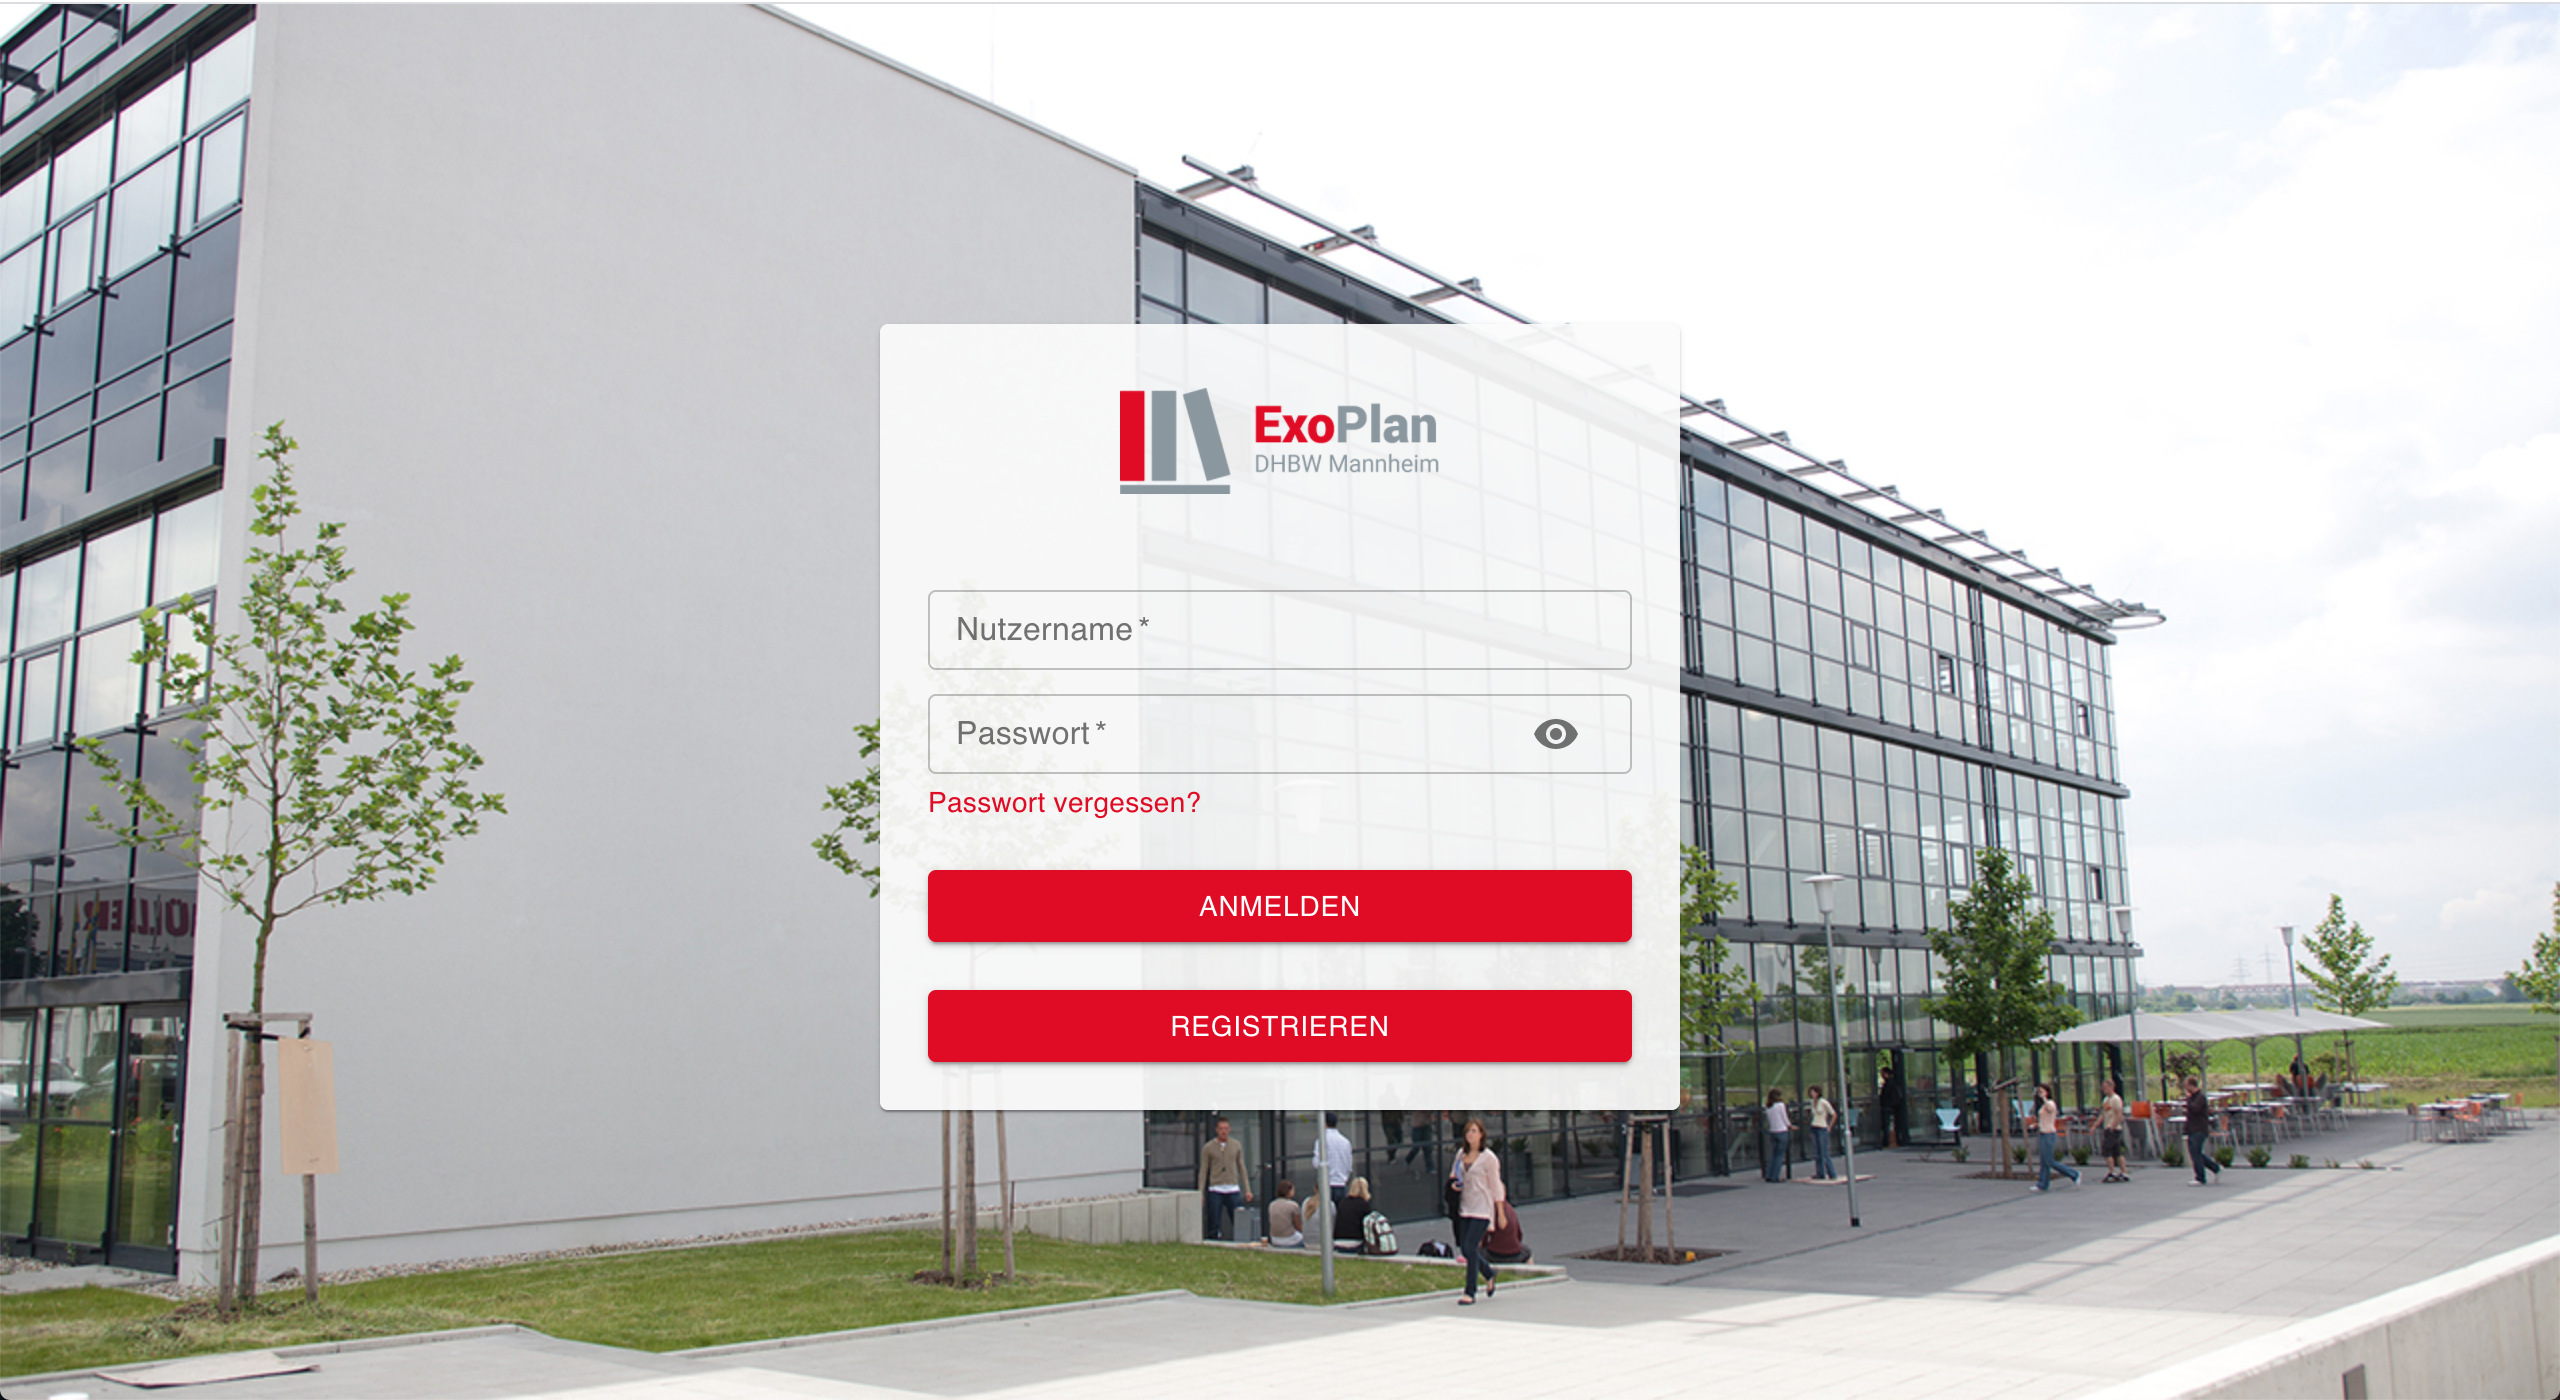
\includegraphics[width=\textwidth]{img/FrontEnd/Login.png}
	\caption[Login]{\label{fig:FE-Login}Login}
\end{figure}

\subsection{Kursübersicht}
Die Hauptansicht der Webanwendung ist die in Abbildung \vref{fig:FE-Vorlesungskalender} dargestellte Seite.
Hier werden die unterschiedlichen Kurse mit den jeweiligen Semestern, den Vorlesungen und dem eingebunden Kurskalendar angezeigt. 
Es können bereits angelegte Kurse verwaltet sowie neue Kurse angelegt werden. 
In Unterkapitel \vref{ch:GC} wird die Einbindung des Kalendars sowie die Verbindung mit dem Google Calendar näher erläutert, da dies eine zentrale Komponente des Front-Ends darstellt.
%TODO Bild erneuern GC
\begin{figure}[H]
	\centering 
	\includegraphics[width=\textwidth]{img/FrontEnd/Vorlesungskalender.png}
	\caption[Kursübersicht mit Vorlesungskalender]{\label{fig:FE-Vorlesungskalender}Kursübersicht mit Vorlesungskalender}
\end{figure}

\subsection{Dozentenansicht}
Unter dem Navigationspunkt \textit{Dozenten} wird der Dozentenpool dargestellt sowie die Möglichkeit zum Hinzufügen von neuen Dozenten gegeben.
Die Umsetzung der Anforderungen A1, A8, A9 und A12 aus Tabelle \vref{anf:Dozenten} ist in Abbildung \vref{fig:FE-Dozenten} zu sehen.
%In Abbildung \vref{fig:FE-DozentenDetail} ist 
Wird ein Dozent ausgewählt, erscheinen weitere Informationen in der Detail-Ansicht. Diese beinhaltet außerdem Funktionen, wie zum Beispiel das Hinterlegen eines Lebenslaufs.
\begin{figure}[H]
	\centering 
	\includegraphics[width=\textwidth]{img/FrontEnd/Dozenten.png}
	\caption[Anzeige der Dozenten]{\label{fig:FE-Dozenten}Anzeige der Dozenten}
\end{figure}
%\begin{figure}[H]
%	\centering 
%	\includegraphics[width=\textwidth]{img/FrontEnd/DozentDetail.png}
%	\caption[Anzeige eines Dozenten]{\label{fig:FE-DozentenDetail}Anzeige eines Dozenten}
%\end{figure}

\subsection{Modulkatalog}
Mit dem Navigationspunkt \textit{Modulkatalog} wird die Anforderungen A4 aus Tabelle \vref{anf:Modulkatalog} umgesetzt. 
Es können Modulkataloge hinzugefügt, angezeigt sowie verwaltet werden. 
\begin{figure}[H]
	\centering 
	\includegraphics[width=\textwidth]{img/FrontEnd/Modulkataloge.png}
	\caption[Anzeige der Modulkatalogen]{\label{fig:FE-Modulkataloge}Anzeige der Modulkatalogen}
\end{figure}

\subsection{Datenverwaltung}
In der Datenverwaltung können die Studiengänge, die Schwerpunkte sowie die Prüfungsleistungen verwaltet werden.
In Abbildung \vref{fig:FE-Datenverwaltung} ist das Hinzufügen, Bearbeiten und Löschen von Studiengängen abgebildet.
\begin{figure}[H]
	\centering 
	\includegraphics[width=\textwidth]{img/FrontEnd/Datenverwaltung.png}
	\caption[Datenverwaltung]{\label{fig:FE-Datenverwaltung}Datenverwaltung}
\end{figure}

\subsection{Administrationsbereich}
Der Administrationsbereich erlaubt es Nutzern mit der Benutzerart \textit{Administrator} andere Benutzer zu verwalten.
Neben dieser Funktionalität, in Abbildung \vref{fig:FE-Administrationsbereich} dargestellt, können Registrierungsschlüssel sowie der Zugang zu dem Google Calendar verwaltet werden.
\begin{figure}[H]
	\centering 
	\includegraphics[width=\textwidth]{img/FrontEnd/Administrationsbereich.png}
	\caption[Administrationsbereich]{\label{fig:FE-Administrationsbereich}Administrationsbereich}
\end{figure}

\subsection{Allgemeine Einstellungen}
Zusätzlich können allgemeine Einstellungen für den Benutzer des Profils verändert werden, die in Abbildung \vref{fig:FE-Einstellungen} dargestellt sind.
So kann der Benutzer unter anderem sein Passwort ändern.
\begin{figure}[H]
	\centering 
	\includegraphics[width=\textwidth]{img/FrontEnd/Einstellungen.png}
	\caption[Allgemeine Kontoeinstellungen]{\label{fig:FE-Einstellungen}Allgemeine Kontoeinstellungen}
\end{figure}



%\subsection{Verwendete Technologie}
%
%Webapplikation basierend auf React (https://reactjs.org/):
%- Grund: Einsteigerfreundlicher als Angular + Vorhaben lässt sich damit gut umsetzen 

%UI Gestaltung mit Material-UI (https://material-ui.com/):
%- Grund: bietet viele nützliche UI Komponenten und Design System für React -> vereinfacht Entwicklung
\section{Test}
Aufgrund der begrenzten Zeit wurde während der Entwicklung hauptsächlich manuell getestet. 
Als weitere Maßnahme zur Qualitätssicherung werden Code Reviews eingesetzt.
Neben Pair Programming sowie Walkthroughs werden hauptsächlich tool-basierte Code Reviews genutzt, indem bei GitHub per Pull Request Feedback von geeigneten anderen Entwicklern zu jeder Codeänderung eingefordert wird.
Dadurch kann die Codequalität sichergestellt sowie Feedback zu den Funktionalitäten eingeholt werden.

Nach Beendigung der Entwicklung wurde außerdem im Front-End ein Abnahmetest von dem Projektergebnis durchgeführt, um die Funktionalitäten zu prüfen sowie einen Abgleich der Benutzeroberfläche durchzuführen. 
Hierbei wurde die Referenzen Design Entwurf aus Kapitel \vref{ch:DesignEntwurf}, der Styleguide im Anhang \vref{an:Styleguide} sowie die Anforderungen der Tabelle \vref{tab:Anforderungen} hinzugezogen.
Dabei wurden mehrere geringfüge Fehler gefunden sowie direkt verbessert. 
Zusätzlich wurden Aspekte festgehalten, die zeitlich nicht mehr geändert sowie umgesetzt werden können, jedoch aber für eine Weiterentwicklung des Produkts von Relevanz sind: 
\begin{itemize}
    \item Hinzufügen eines Lebenslaufs von einem Dozenten sowie erlaubte Formate und maximale Dateigröße bestimmen
    \item Löschen von Modulkatalogen 
    \item Entzug von Administrationsrechten
    \item Studiengangsrichtung nur bei zutreffenden Studiengängen (z.B. der Studiengang Digitale Medien hat keine Studienrichtungen)
    \item Hinzufügen von Vorlesungsinformationen zu den Kalendareinträgen.
\end{itemize}
\chapter{User Guide}
\label{ch:UserGuide}
\section{Setup}
\subsection{Repositories von GitHub clonen}

Das Projekt Exoplan setzt sich aus einem Frontend und einem Backend zusammen. Diese sind jeweils in ein eigenes Repository ausgelagert und müssen einzeln ausgecheckt werden. Dazu ist es empfehlenswert ein Verzeichnis mit dem Namen \texttt{dhbw-projekt} anzulegen. Folgende Repositories gilt es auszuchecken:
\begin{itemize}
	\item https://github.com/nikolockenvitz/dhbw-project-frontend
	\item https://github.com/nikolockenvitz/dhbw-project-backend
\end{itemize}

Zum Auschecken werden die folgenden Befehle verwendet:

\texttt{git clone https://github.com/nikolockenvitz/dhbw-project-frontend.git}

\texttt{git clone https://github.com/nikolockenvitz/dhbw-project-backend.git}

\subsection{Konfiguration von Backend}

Um das Backend verwenden zu können, ist es notwendig \textit{Docker} zu installieren, falls dies noch nicht installiert ist. Die korrekte Funktion von Docker kann mit dem folgenden Befehl überprüft werden: \texttt{docker version}.

Wenn \textit{Docker} korrekt funktioniert, sind weitere Konfigurationen notwendig:

\begin{enumerate}
	\item Im Root-Verzeichnis muss das Verzeichnis \texttt{env} angelegt werden.
	\item Im \texttt{env}-Verzeichnis wird die Datei \texttt{app.properties} mit dem folgenden Inhalt angelegt:
	\begin{lstlisting}
	app.port = 3000
	app.defaultUser = admin
	app.defaultPassword = defaultpasswordhere
	app.isAdmin = true
	app.forceSync = false
	app.enableTestData = false
	
	server.user     = dhbw
	server.database = becker
	server.password = iH0p3youU5EaSecretPa$$word
	server.port = 5432
	server.dialect = postgres
	jwt.superSecret = TreevgQreNefpuUngHroreunhcg
	AvpugfTrznpug13
	server.host = postgres
	
	pepper = ErarFgvaxg
	\end{lstlisting}
	
	\item Im Verzeichnis \texttt{./docker} wird die Datei \texttt{.env} angelegt. Dort werden weitere Konfigurationen für die Verwendung der Datenbank vorgenommen:
	
	\begin{lstlisting}
	postgres_user=dhbw
	postgres_password=iH0p3youU5EaSecretPa$$word
	postgres_port=5432
	pgadmin_user=project@dhbw.de
	pgadmin_password=test1234
	\end{lstlisting}
	
	\item Im nächsten Schritt müssen die benötigten Zertifikate in das Verzeichnis \texttt{./docker
		/nginx/ssl} kopiert werden.
	
\end{enumerate}

\subsection{Start von Exoplan}

Da für das Frontend keine Konfiguration vorgenommen werden muss, kann nun das  Gesamtsystem gestartet werden. Hierfür wird im Backend-Verzeichnis in das Verzeichnis \texttt{./docker} navigiert und der folgende Befehl ausgeführt: \texttt{docker-compose up --build}

Nach einem erfolgreichen Start kann Exoplan über \textit{https://localhost/} aufgerufen werden. Der Administrator kann sich nun mit dem Benutzer \texttt{admin} und dem Passwort \texttt{test} anmelden. Diese Anmeldedaten sollte anschließend sofort geändert werden.

Wenn Exoplan kann des Weiteren über den folgenden Befehl heruntergefahren werden. Achtung: Hierfür muss in das Backend-Verzeichnis und dem darin befindlichen \texttt{./docker}-Verzeich navigiert werden:

\texttt{docker-compose down}

%\begin{itemize}
%	\item Wie bekommt man das Projekt? / Woraus besteht das Paket?
%	\item Was muss man tun, um die Web-Anwendung aufzusetzen? 
%	\item Welche Konfigurationen müssen vorgenommen werden?
%	\item Was sind die Login-Daten? 
%	\item VM, Docker
%\end{itemize}

\section{Funktionalitäten}
%TODO Trello-Hinweis über Farben des Status auf Vorlesungspläne: \url{https://trello.com/c/ciMzmZTX}

In diesem Abschnitt soll eine grobe Übersicht über die Hauptfunktionalitäten von Exoplan gegeben werden. Diese sind nachfolgend aufgelistet und werden mit Hilfe von Beispielen erklärt.

Grobe Übersicht über die Hauptprozesse, wie: 
%Keine Screenshots sondern wir läuft der Prozess ab
\begin{itemize}
	\item Neuen Kurs anlegen,
	\item Dozenten kontaktieren (Status nutzen),
	\item Vorlesungen im Kalender verwalten,
	\item Modulkatalog verwalten,
	\item Datenverwaltung - Studiengänge, Schwerpunkte, Prüfungsleistungen,
	\item Administration - Registrierungsschlüssel, Benutzer, Google-Calendar.
\end{itemize}

\subsection{Neuen Kurs anlegen}

Um einen Kurs neuen in Exoplan anzulegen, muss sich der Benutzer mit seinen Anmeldedaten anmelden. Anschließen kann in der Anwendung auf der linken Seite der Menüpunkt \textit{Verlesungspläne} ausgewählt werden. Daraufhin wird der Tab \textit{Kurs hinzufügen} dargestellt, welcher daraufhin geöffnet wird.

Damit das volle Potential des Exoplan-System vollumfänglich ausgeschöpft werden kann, muss die Kurskonfiguration sehr genau durchgeführt werden. Hierbei wird zuerst der Name des Kurses angegeben, also zum Beispiel \textit{WWI17SEB}. Außerdem müssen Studiengang (Wirtschaftinformatik, BWL, usw.) und Studienrichtung (Software Engineering, Sales and Consulting) für den Kurs spezifiziert werden. Abschließend wird die Anzahl der Semester ausgewählt, der Zeitraum für jedes Semester angegeben und die Google Calender ID des Kurses eingetragen.

\subsection{Dozenten kontaktieren}

Im Studienalltag gilt es viele verschiedene Informationen gleichzeitig zu bewältigen. Ein großes Problem ist hierbei eine Überblick über die vorhandenen Dozenten und ihrer Expertise zu behalten. Aus diesem Grund bietet Exoplan eine leistungsstarke und zugleich einfache Dozentenverwaltung. Diese Kann 

\subsection{Vorlesungen im Kalender verwalten}



\subsection{Modulkatalog verwalten}

Auch Modulkataloge lassen sich in Exoplan verwalten, speichern und anpassen. Diese bilden die Grundlage für die Planung von Vorlesungen und gesanten Studienablaufs in Exoplan. Dazu wird der Menüpunkt \textit{Modulkataloge} auf der linken Seite ausgwählt. Anschließend werden alle vorhandenen Modulkataloge angezeigt. Des Weiteren kann ein neuer Modulkatalog durch einen Klick auf den Button \textit{Modulkatalog Hinzufügen} erstellt werden. 

Auch kann ein Modulkatalog durch eine einfache Auswahl geöffnet werden. Hierbei werden anschließen alle dazugehörenden Module angezeigt. Auch lassen sich Module bearbeiten und löschen.

\subsection{Administrationsbereich}

Im Administrationsbereich können verschiedene Einstellungen vorgenommen werden, um den Betrieb von Exoplan zu gewährleisten. Der Administrationsbereich kann durch den Menüpunkt \textit{Administrationsbereich} aufgerufen werden.

\subsubsection{Benutzerverwaltung}

Die Benutzerverwaltung kann über den Tab \textit{Benutzer} erreicht werden und liefert eine Übersicht über alle im System registrierten Benutzer. Es werden Informationen zur Art des Benutzers (Administrator, Studiengangsleiter und Benutzer) und der Passwortstatus (OK, Wechsel erforderlich) angegeben. Des Weiteren kann in dieser Übersicht ein Studiengangsleiter angelegt und auch ein Passwortreset durchgeführt werden.

\subsubsection{Registrierungschlüssel}

Registrierungsschlüssel werden benötigt, damit sich neue Benutzer in Exoplan registrieren können. Dieser Schlüssel kann über den Tab \textit{Registrierungschlüssel} festgelegt werden.

\subsubsection{Google Calender}

\chapter{Evaluation}

\section{Bewertung Umsetzung}
\begin{itemize}
	\item Abgleich Anforderungen
	\item Derzeitiger Stand der Software
\end{itemize}
\section{Lessons Learned}
Während der Arbeit an dem Projekt wurden viele Erkenntnisse gewonnen, neues Wissen erlangt sowie wertvolle Erfahrungen gesammelt.
Zunächst lässt sich festhalten, dass die Projektmitglieder viel technische als auch organisatorische Aspekte gelernt haben.
Im Folgenden werden drei Lessons Learned näher erläutert, die Optimierungspotenziale während oder nach dem Projekt bereitgehalten haben.
\subsection{Kommunikation}
Eine Herausforderung, die in jedem Gruppenprojekt zu meistern ist, ist die Kommunikation zwischen den Projektmitgliedern erfolgreich zu gestalten. 
Hierbei war eine besondere Hürde auch die Gruppengröße, die ein zusätzlicher Faktor für die Koordination und die Absprachen war. 
Ein respektvoller Umgang zwischen den Projektmitgliedern ist sehr wichtig und beeinflusst den Projektverlauf.
Während des Projektverlaufs wurde die Erkenntnis gezogen, dass eine verstärkte Kommunikation in den Teams sich positiv auf den Fortschritt auswirkt. 
Diese Optimierungsmöglichkeit wurde nach einer Reflexion des 5. Semesters gezogen und somit im 6. Semester verbessert. 

\subsection{Inhaltliche Ziele mit festen Milestones}
Wie bereits in der \hyperref[ch:zeitplanung]{Zeitplanung} ersichtlich, wurden in dem 6. Semester auch inhaltliche Ziele festgelegt. 
Diese Vorgehensweise hat sich als zielführender herausgestellt, da der Projektverlauf dadurch besser kontrolliert sowie die Umsetzung besser geplant werden konnte.
Auch für das 5. Semester wäre dies von Vorteil gewesen und wird als Erfahrung aus dem Projekt mitgenommen.

\subsection{Punktesystem}
Zur Bewertung der Leistung der Projektmitglieder wurde der Aufwand als Ist-Stunden verwendet sowie vergütet.
Da sich das Projektteam aus Personen mit unterschiedlichen Kompetenzen zusammensetzt, wurde oft in Kleingruppen zusammengearbeitet. 
Hierbei haben unter anderem Mitglieder mit höherer Expertise anderen Projektmitgliederns ausgeholfen.
Beide Personen haben jedoch den gleichen Aufwand bekommen, sodass dies von den Mitgliedern mit tiefergreifendem Wissensstand als unfaire Lösung angesehen wurde. 
Zusätzlich hat sich im Laufe des Projekts herausgestellt, dass es Projektmitglieder gibt, die das Projektergebnis maßgeblich vorangetrieben haben.
Um diese Leistung sowie die eingebrachte Expertise zu honorieren, wäre es möglich ein Bonussystem einzuführen. 
Dieses würde es ermöglichen, den entsprechenden Personen einen Bonus zu vergeben und entsprechend die Leistung zu vergüten.

Das Bewertungssystem hat sich während des  Projekts als strittiger Punkt herausgestellt, da es trotz Änderungen von einigen als unfair empfunden wird.
Dort ist allerdings festzuhalten, dass es besonders bei einer solchen Gruppengröße, sehr herausfordernd ist es allen Recht zu machen.

\section{Nächste Schritte}
\begin{itemize}
	\item Erweiterbarkeit
\end{itemize}
\chapter{Fazit und Ausblick}
\section{Fazit}
Abschließend lässt sich sagen, dass das Projekt sehr erfolgreich abgeschlossen werden konnte. 
Wie in Tabelle \vref{tab:erfanf} ersichtlich wurden alle Muss-Anforder"-ungen und circa die Hälfte der Kann-Anforderungen erfüllt.
Bei dem Projektteam war allgemein eine gute Arbeitsmoral von Projektbeginn bis -ende spürbar.
Jedes Teammitglied konnte und hat seine Fähigkeiten einbringen können und etwas zu dem Projekterfolg beigetragen.
Dies ist auch aus den Bewertungspunkten ersichtlich,die kaum Ausreißer nach unten aufweisen.
Während des Projekts konnten bereits mehrere Dinge verbessert werden. 
Dazu zählt die Zeitplanung des 6. Semesters, welche zu den jeweiligen zeitlichen Abschnitten inhaltliche Ziele beinhaltet, sodass der Fortschritt der Entwicklung besser überprüft werden konnte.
Eine weitere Verbesserung bestand in der Kommunikation.
Es wurde generell verstärkt kommuniziert, sowohl im gesamten Team, den jeweiligen Untergruppen als auch mit den Leitern des Projekts. 
Wichtig zu erwähnen ist auch, dass das durch COVID-19 bedingte Online-Semester kein Hindernis für die Umsetzung des Projekts darstellte.
Die Absprachen sowie das kollaborative Entwickeln konnten über das verwendete Konferenzsystem verteilt stattfinden.

\section{Ausblick}
Das Endprodukt bietet noch Möglichkeiten zur weiteren Entwicklung. 
Im Folgenden werden mögliche Schritte zur Erweiterung aufgeführt.
Dazu zählen hauptsächlich die noch nicht umgesetzten Kann-Anforderungen, welche der Tabelle \vref{tab:erfanf} entnommen werden können.
Außerdem wurden durch den Abnahmetest in Kapitel \vref{ch:Test} zusätzliche Möglichkeiten zur Erweiterung aufgezeigt.

Die im Folgenden beschriebenen Punkte sind ebenfalls für die zukünftige Verwendung des Tools zu berücksichtigen.
Für die Entwicklung der Anwendung wurden selbstsignierte Zertifikate verwendet, die vor der Verwendung ausgetauscht werden sollten.
Außerdem sind nicht alle entwickelten Routen komplett nach dem REST-Paradigma erstellt, wodurch dort eine weitere Möglichkeit zur Verbesserung besteht.
Für den laufenden Betrieb ist außerdem zu beachten, dass die Datenbank in einem Docker-Container läuft und deshalb nur so lange persistiert ist, wie der Container ohne Unterbrechung hochgefahren ist.
Aus diesem Grund sollten regelmäßige Backups durchgeführt oder der Container auf eine persistente Schicht gemountet werden. 
Des Weiteren werden Passwörter in der Anwendung als Hashwert gespeichert.
Eine Verbesserungsmöglichkeit ist den Hashwert direkt Clientseitig zu bilden, damit Passwörter nie im Klartext an den Server übermittelt werden.


%	Literaturverzeichnis
% \printbibliography[title=Literaturverzeichnis]
% \cleardoublepage

% Der Anhang beginnt hier - jedes Kapitel wird alphabetisch aufgezählt. (Anhang A, B usw.)
% \appendix
% \ihead{\appendixname~\thechapter} % Neue Header-Definition

% appendix.tex einziehen
% \chapter{Abbildungen}
\begin{figure}[h]
	\centering 
	\includegraphics[angle={90}, width=\textwidth]{img/er-model.pdf}
	\captionsetup{format=hang}
	\caption[Entity-Relationship-Modell]{\label{fig:ermodell}ER-Modell}
\end{figure}




\end{document}